\chapter{Networking e Volumes}

\section*{Introduzione}
Il networking e la gestione dei volumi sono fondamentali per container che devono comunicare tra loro e persistere dati. Questo capitolo esplora i diversi driver di rete Docker, il service discovery, e le strategie di gestione volumi per garantire persistenza e backup.

\section*{Obiettivi di apprendimento}
\begin{itemize}
    \item Comprendere i driver di rete: bridge, host, overlay, none
    \item Creare reti custom e isolare container
    \item Configurare port mapping e service discovery
    \item Gestire volumi per persistenza dati
    \item Implementare backup e restore di volumi
    \item Usare bind mounts e tmpfs appropriatamente
\end{itemize}

\section{Docker Networking}

\subsection{Concetti Fondamentali}

Docker usa \textbf{network drivers} per fornire networking ai container:
\begin{itemize}
    \item \textbf{bridge}: Default, rete privata su un singolo host
    \item \textbf{host}: Usa direttamente il network stack dell'host
    \item \textbf{overlay}: Multi-host networking (Swarm/Kubernetes)
    \item \textbf{macvlan}: Assegna MAC address ai container
    \item \textbf{none}: Nessun networking
\end{itemize}

\subsection{Comandi Base}

\begin{lstlisting}[language=bash]
# Lista reti
$ docker network ls
NETWORK ID     NAME      DRIVER    SCOPE
abc123def456   bridge    bridge    local
123456789abc   host      host      local
def456abc123   none      null      local

# Crea rete custom
$ docker network create mynetwork
$ docker network create --driver bridge my-bridge-net

# Ispeziona rete
$ docker network inspect mynetwork

# Connetti container a rete
$ docker network connect mynetwork container1

# Disconnetti
$ docker network disconnect mynetwork container1

# Rimuovi rete
$ docker network rm mynetwork

# Pulisci reti non usate
$ docker network prune
\end{lstlisting}

\section{Bridge Network}

\subsection{Default Bridge}

Quando avvii un container senza specificare \texttt{--network}, usa la rete \texttt{bridge} di default.

\begin{lstlisting}[language=bash, caption=Container su bridge default]
# Avvia due container
$ docker run -d --name container1 alpine sleep 1000
$ docker run -d --name container2 alpine sleep 1000

# Verifica network
$ docker inspect container1 | jq '.[0].NetworkSettings.Networks'
{
  "bridge": {
    "IPAddress": "172.17.0.2",
    ...
  }
}

# Comunicazione via IP (funziona)
$ docker exec container1 ping -c 2 172.17.0.3
PING 172.17.0.3 (172.17.0.3): 56 data bytes
64 bytes from 172.17.0.3: seq=0 ttl=64 time=0.123 ms

# Comunicazione via nome (NON funziona su default bridge!)
$ docker exec container1 ping container2
ping: bad address 'container2'
\end{lstlisting}

\textbf{Limitazioni default bridge}:

Il bridge di default presenta alcune limitazioni significative che ne sconsigliano l'uso in ambienti di produzione. L'assenza di automatic service discovery basato su DNS costringe i container a comunicare tramite indirizzi IP hardcoded, rendendo la configurazione fragile e difficile da mantenere. La comunicazione è possibile esclusivamente via IP, eliminando la possibilità di riferirsi ai container tramite nomi simbolici. Inoltre, tutti i container connessi al bridge di default possono vedere e comunicare con tutti gli altri, mancando di granularità nel controllo dell'isolamento di rete.

\subsection{User-Defined Bridge}

\textbf{Best practice}: Usa sempre reti custom per service discovery automatico.

\begin{lstlisting}[language=bash, caption=Custom bridge network]
# Crea rete custom
$ docker network create --driver bridge my-app-net

# Avvia container su rete custom
$ docker run -d --name web --network my-app-net nginx
$ docker run -d --name db --network my-app-net postgres

# Service discovery via DNS (funziona!)
$ docker exec web ping -c 2 db
PING db (172.18.0.3): 56 data bytes
64 bytes from 172.18.0.3: seq=0 ttl=64 time=0.089 ms

# Inspect network
$ docker network inspect my-app-net
[
    {
        "Name": "my-app-net",
        "Driver": "bridge",
        "Containers": {
            "abc123": {
                "Name": "web",
                "IPv4Address": "172.18.0.2/16"
            },
            "def456": {
                "Name": "db",
                "IPv4Address": "172.18.0.3/16"
            }
        }
    }
]
\end{lstlisting}

\subsection{Configurazione Bridge Avanzata}

\begin{lstlisting}[language=bash, caption=Opzioni custom bridge]
# Subnet e gateway custom
$ docker network create \
  --driver bridge \
  --subnet 192.168.100.0/24 \
  --gateway 192.168.100.1 \
  --ip-range 192.168.100.0/25 \
  my-custom-net

# IP statico per container
$ docker run -d \
  --name web \
  --network my-custom-net \
  --ip 192.168.100.10 \
  nginx
\end{lstlisting}

\section{Host Network}

Il container usa direttamente il network stack dell'host, senza isolamento.

\begin{lstlisting}[language=bash, caption=Host network mode]
# Container usa network dell'host
$ docker run -d --name nginx-host --network host nginx

# Nginx ascolta su porta 80 dell'HOST (non del container)
$ curl http://localhost:80
<!DOCTYPE html>
<html>
<title>Welcome to nginx!</title>
...

# No port mapping necessario (-p non serve)
\end{lstlisting}

\textbf{Vantaggi}:

L'uso della host network offre benefici tangibili in termini di performance, eliminando completamente l'overhead del NAT (Network Address Translation) e permettendo al container di operare con latenza minima. Il container ottiene inoltre accesso diretto a tutte le interfacce di rete dell'host, facilitando scenari in cui è necessario interagire con hardware di rete specifico o monitorare tutto il traffico della macchina.

\textbf{Svantaggi}:

Questi vantaggi hanno un costo elevato in termini di sicurezza e gestibilità. L'assenza totale di isolamento di rete espone l'host a potenziali rischi se il container viene compromesso. Si creano inevitabili conflitti di porta quando più container tentano di utilizzare la stessa porta, rendendo impossibile eseguire repliche multiple dello stesso servizio. Inoltre, questa modalità non è supportata su Docker Desktop per macOS e Windows, limitandone l'applicabilità in ambienti di sviluppo cross-platform.

\textbf{Quando usarlo}:

L'host network è appropriato per scenari specifici dove le performance sono assolutamente critiche, come sistemi di monitoring che devono analizzare tutto il traffico di rete con latenza minimale, o load balancer ad alte prestazioni. È inoltre indicato per container che devono gestire direttamente l'intero stack di networking dell'host, come soluzioni VPN o firewall che richiedono controllo completo sulle interfacce di rete.

\section{Overlay Network}

Per multi-host networking (Docker Swarm, Kubernetes).

\begin{lstlisting}[language=bash, caption=Overlay network (Swarm mode)]
# Inizializza Swarm
$ docker swarm init

# Crea overlay network
$ docker network create \
  --driver overlay \
  --attachable \
  my-overlay-net

# Deploy servizio su overlay
$ docker service create \
  --name web \
  --network my-overlay-net \
  --replicas 3 \
  nginx

# Container su host diversi possono comunicare
\end{lstlisting}

\textbf{Caratteristiche}:
\begin{itemize}
    \item Comunicazione tra container su host fisici diversi
    \item Encryption opzionale del traffico
    \item Service discovery integrato
    \item Load balancing automatico
\end{itemize}

\section{None Network}

Nessun networking, completo isolamento.

\begin{lstlisting}[language=bash]
# Container isolato
$ docker run -d --name isolated --network none alpine sleep 1000

# Verifica: solo loopback
$ docker exec isolated ip addr show
1: lo: <LOOPBACK,UP,LOWER_UP> mtu 65536
    inet 127.0.0.1/8 scope host lo
\end{lstlisting}

\textbf{Quando usarlo}:
\begin{itemize}
    \item Elaborazione dati sensibili senza accesso rete
    \item Testing isolato
    \item Container che comunicano solo via volumi condivisi
\end{itemize}

\section{Port Mapping}

\subsection{Pubblicare Porte}

\begin{lstlisting}[language=bash]
# Porta specifica: host:container
$ docker run -d -p 8080:80 nginx

# Porta random host
$ docker run -d -p 80 nginx
$ docker ps  # Vedi porta assegnata (es. 0.0.0.0:32768->80/tcp)

# Multiple porte
$ docker run -d \
  -p 8080:80 \
  -p 8443:443 \
  nginx

# IP specifico host
$ docker run -d -p 127.0.0.1:8080:80 nginx

# UDP
$ docker run -d -p 53:53/udp dns-server
\end{lstlisting}

\subsection{Port Binding vs Expose}

\begin{lstlisting}[caption=Differenza EXPOSE vs -p]
# Dockerfile: EXPOSE documenta porta
EXPOSE 80

# Run: -p pubblica effettivamente
$ docker run -p 8080:80 myapp

# Senza -p, porta non accessibile dall'host
$ docker run myapp  # Porta 80 non raggiungibile esternamente
\end{lstlisting}

\section{Service Discovery}

\subsection{DNS Automatico}

Su reti custom, Docker fornisce DNS automatico.

\begin{lstlisting}[language=bash, caption=Service discovery example]
# Crea rete
$ docker network create app-net

# Servizio backend
$ docker run -d \
  --name api \
  --network app-net \
  myapi

# Servizio frontend può chiamare backend via nome
$ docker run -d \
  --name frontend \
  --network app-net \
  -e API_URL=http://api:3000 \
  myfrontend

# Frontend può risolvere "api" via DNS
$ docker exec frontend nslookup api
Server:  127.0.0.11
Address: 127.0.0.11:53

Name:    api
Address: 172.20.0.2
\end{lstlisting}

\subsection{Network Aliases}

\begin{lstlisting}[language=bash]
# Multipli alias per stesso container
$ docker run -d \
  --name db \
  --network app-net \
  --network-alias database \
  --network-alias postgres \
  postgres

# Raggiungibile via db, database, o postgres
$ docker exec frontend ping database
$ docker exec frontend ping postgres
\end{lstlisting}

\section{Isolamento e Sicurezza}

\subsection{Reti Multiple}

\begin{lstlisting}[language=bash, caption=Segmentare applicazione]
# Rete frontend
$ docker network create frontend-net

# Rete backend (internal, no internet)
$ docker network create --internal backend-net

# Frontend: accessibile esternamente
$ docker run -d \
  --name web \
  --network frontend-net \
  -p 80:80 \
  nginx

# API: su entrambe le reti
$ docker run -d \
  --name api \
  --network frontend-net \
  nginx-api

$ docker network connect backend-net api

# Database: solo backend (non raggiungibile da internet)
$ docker run -d \
  --name db \
  --network backend-net \
  postgres
\end{lstlisting}

\textbf{Architettura}:
\begin{verbatim}
Internet
   |
[web] ----+
          |
      [frontend-net]
          |
        [api]
          |
      [backend-net]
          |
        [db]
\end{verbatim}

\subsection{Firewall e IPTables}

Docker modifica automaticamente iptables per port mapping.

\begin{lstlisting}[language=bash]
# Visualizza regole Docker
$ sudo iptables -t nat -L -n

# Disabilita modifica iptables (daemon.json)
{
  "iptables": false
}
\end{lstlisting}

\section{Docker Volumes}

\subsection{Tipi di Persistenza}

\begin{enumerate}
    \item \textbf{Volumes}: Gestiti da Docker, best practice
    \item \textbf{Bind mounts}: Directory host montate nel container
    \item \textbf{tmpfs mounts}: Memoria RAM, non persistente
\end{enumerate}

\begin{figure}[h]
    \centering
    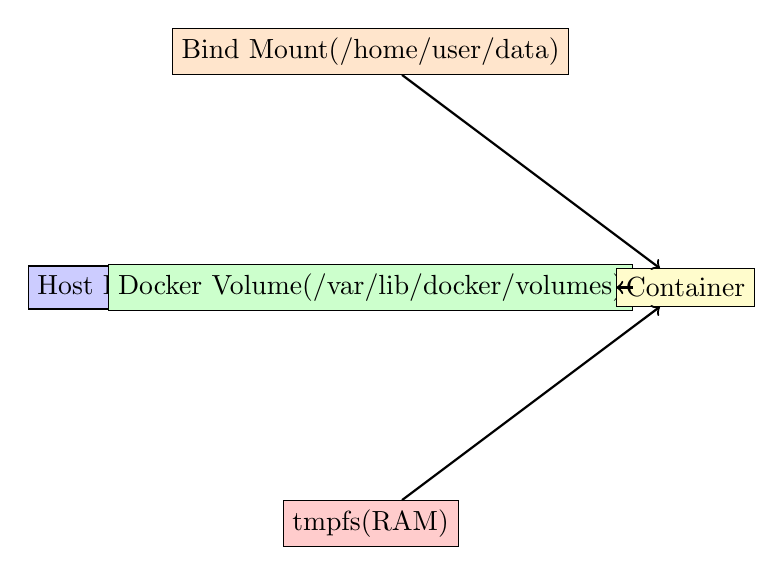
\begin{tikzpicture}[node distance=3cm]
        \node[draw, rectangle, fill=blue!20] (host) {Host Filesystem};
        \node[draw, rectangle, fill=green!20, right of=host] (volume) {Docker Volume\\(/var/lib/docker/volumes)};
        \node[draw, rectangle, fill=orange!20, above of=volume] (bind) {Bind Mount\\(/home/user/data)};
        \node[draw, rectangle, fill=red!20, below of=volume] (tmpfs) {tmpfs\\(RAM)};

        \node[draw, rectangle, fill=yellow!20, right of=volume, node distance=4cm] (container) {Container};

        \draw[->, thick] (volume) -- (container);
        \draw[->, thick] (bind) -- (container);
        \draw[->, thick] (tmpfs) -- (container);
    \end{tikzpicture}
    \caption{Tipi di mount in Docker}
\end{figure}

\subsection{Named Volumes}

\begin{lstlisting}[language=bash]
# Crea volume
$ docker volume create mydata

# Lista volumi
$ docker volume ls
DRIVER    VOLUME NAME
local     mydata

# Ispeziona
$ docker volume inspect mydata
[
    {
        "Name": "mydata",
        "Driver": "local",
        "Mountpoint": "/var/lib/docker/volumes/mydata/_data",
        "Labels": {},
        "Scope": "local"
    }
]

# Usa in container
$ docker run -d \
  --name db \
  -v mydata:/var/lib/postgresql/data \
  postgres

# Rimuovi volume
$ docker volume rm mydata

# Pulisci volumi non usati
$ docker volume prune
\end{lstlisting}

\subsection{Bind Mounts}

\begin{lstlisting}[language=bash]
# Mount directory host
$ docker run -d \
  --name web \
  -v /home/user/html:/usr/share/nginx/html \
  nginx

# Path relativo (PWD)
$ docker run -d \
  --name app \
  -v $(pwd)/app:/app \
  myapp

# Read-only mount
$ docker run -d \
  --name web \
  -v $(pwd)/html:/usr/share/nginx/html:ro \
  nginx

# Sintassi --mount (più esplicita)
$ docker run -d \
  --mount type=bind,source=$(pwd)/app,target=/app \
  myapp
\end{lstlisting}

\textbf{Bind Mounts vs Volumes}:

\begin{table}[h]
\centering
\begin{tabular}{|l|l|l|}
\hline
\textbf{Aspetto} & \textbf{Bind Mount} & \textbf{Volume} \\
\hline
Path & Host filesystem & Docker area \\
Gestione & Manuale & Docker \\
Performance & Buona & Ottima (Linux) \\
Portabilità & Bassa & Alta \\
Backup & Manuale & Docker CLI \\
Uso & Sviluppo & Produzione \\
\hline
\end{tabular}
\caption{Bind Mount vs Volume}
\end{table}

\subsection{tmpfs Mounts}

Dati in RAM, non scritti su disco.

\begin{lstlisting}[language=bash]
# Mount tmpfs
$ docker run -d \
  --name tmptest \
  --tmpfs /app/cache:rw,size=100m \
  myapp

# Sintassi --mount
$ docker run -d \
  --mount type=tmpfs,target=/app/cache,tmpfs-size=100m \
  myapp
\end{lstlisting}

\textbf{Quando usare tmpfs}:
\begin{itemize}
    \item Dati sensibili (credenziali temporanee)
    \item Cache ad alte performance
    \item File temporanei che non devono persistere
\end{itemize}

\section{Gestione Avanzata Volumi}

\subsection{Volume Drivers}

\begin{lstlisting}[language=bash]
# Driver locale (default)
$ docker volume create --driver local myvolume

# NFS volume
$ docker volume create \
  --driver local \
  --opt type=nfs \
  --opt o=addr=192.168.1.1,rw \
  --opt device=:/path/to/dir \
  nfs-volume

# Cloud storage (plugin richiesto)
$ docker volume create \
  --driver rexray/s3fs \
  --opt=size=20 \
  s3-volume
\end{lstlisting}

\subsection{Backup e Restore}

\begin{lstlisting}[language=bash, caption=Backup volume]
# Backup volume in tar.gz
$ docker run --rm \
  -v mydata:/data \
  -v $(pwd):/backup \
  alpine \
  tar czf /backup/mydata-backup.tar.gz -C /data .

# Verifica backup
$ ls -lh mydata-backup.tar.gz
-rw-r--r-- 1 user user 1.5M Nov 15 10:00 mydata-backup.tar.gz
\end{lstlisting}

\begin{lstlisting}[language=bash, caption=Restore volume]
# Crea nuovo volume
$ docker volume create mydata-restored

# Restore da backup
$ docker run --rm \
  -v mydata-restored:/data \
  -v $(pwd):/backup \
  alpine \
  sh -c "cd /data && tar xzf /backup/mydata-backup.tar.gz"
\end{lstlisting}

\subsection{Condivisione Volumi tra Container}

\begin{lstlisting}[language=bash]
# Container 1 scrive dati
$ docker run -d \
  --name writer \
  -v shared-data:/data \
  alpine \
  sh -c "while true; do date >> /data/log.txt; sleep 5; done"

# Container 2 legge dati
$ docker run -d \
  --name reader \
  -v shared-data:/data:ro \
  alpine \
  sh -c "tail -f /data/log.txt"

# Verifica
$ docker logs reader
Wed Nov 15 10:00:00 UTC 2025
Wed Nov 15 10:00:05 UTC 2025
...
\end{lstlisting}

\subsection{Volumes from Container}

\begin{lstlisting}[language=bash]
# Data container
$ docker create -v /data --name data-container alpine

# App usa volumi da data-container
$ docker run -d \
  --name app1 \
  --volumes-from data-container \
  myapp

$ docker run -d \
  --name app2 \
  --volumes-from data-container \
  myapp
\end{lstlisting}

\section{Esempi Pratici}

\subsection{Database con Persistenza}

\begin{lstlisting}[language=bash, caption=PostgreSQL production setup]
# Crea rete e volume
$ docker network create db-net
$ docker volume create postgres-data

# Deploy PostgreSQL
$ docker run -d \
  --name postgres \
  --network db-net \
  --restart unless-stopped \
  -e POSTGRES_PASSWORD=secret \
  -v postgres-data:/var/lib/postgresql/data \
  -v $(pwd)/init.sql:/docker-entrypoint-initdb.d/init.sql:ro \
  postgres:15

# Backup automatico (cron job)
$ docker run --rm \
  --network db-net \
  -v postgres-data:/data \
  -v $(pwd)/backups:/backups \
  postgres:15 \
  pg_dump -h postgres -U postgres -F c -f /backups/db-$(date +%Y%m%d).dump
\end{lstlisting}

\subsection{Sviluppo con Hot Reload}

\begin{lstlisting}[language=bash, caption=Node.js development]
# Bind mount per hot reload
$ docker run -d \
  --name node-dev \
  -p 3000:3000 \
  -v $(pwd)/app:/usr/src/app \
  -v /usr/src/app/node_modules \
  -e NODE_ENV=development \
  node:18 \
  npm run dev

# Modifiche a app/ si riflettono immediatamente
\end{lstlisting}

\subsection{Multi-Tier App Networking}

\begin{lstlisting}[language=bash, caption=3-tier architecture]
# Reti
$ docker network create frontend-net
$ docker network create backend-net

# Database (solo backend)
$ docker run -d \
  --name db \
  --network backend-net \
  -v db-data:/var/lib/postgresql/data \
  postgres

# API (frontend + backend)
$ docker run -d \
  --name api \
  --network frontend-net \
  -e DB_HOST=db \
  node-api

$ docker network connect backend-net api

# Web (solo frontend)
$ docker run -d \
  --name web \
  --network frontend-net \
  -p 80:80 \
  nginx
\end{lstlisting}

\section*{Best Practices}

\begin{tcolorbox}[colback=yellow!10, colframe=orange!60, title=Best Practices]
\textbf{Networking}:
\begin{itemize}
    \item Usa reti custom per service discovery automatico
    \item Segmenta applicazione con reti multiple
    \item Usa \texttt{--internal} per reti senza accesso internet
    \item Evita \texttt{--network host} se non necessario
    \item Documenta port mapping nei README
\end{itemize}

\textbf{Volumes}:
\begin{itemize}
    \item Named volumes in produzione, bind mounts in sviluppo
    \item Backup regolari di volumi critici
    \item Usa \texttt{:ro} per mount read-only quando possibile
    \item Pulisci volumi inutilizzati periodicamente
    \item Considera driver cloud per high availability
\end{itemize}
\end{tcolorbox}

\section*{Errori Comuni}

\begin{attenzione}
\begin{enumerate}
    \item \textbf{Default bridge senza DNS}: Usa reti custom

    \item \textbf{Porta in conflitto}:
    \begin{lstlisting}
Error: Bind for 0.0.0.0:80 failed: port is already allocated
    \end{lstlisting}
    Soluzione: Cambia porta host o ferma servizio esistente

    \item \textbf{Volume cancellato per errore}:
    \begin{lstlisting}
$ docker compose down -v  # ATTENZIONE: cancella volumi!
    \end{lstlisting}
    Soluzione: Ometti -v, usa backup regolari

    \item \textbf{Bind mount con path errato}: Verifica path assoluti

    \item \textbf{Permission denied su bind mount}: Controlla ownership/chmod

    \item \textbf{Container non comunicano}: Verifica stessa rete
\end{enumerate}
\end{attenzione}

\section*{Esercizi}

\begin{enumerate}
    \item Crea un'app WordPress:
    \begin{itemize}
        \item MySQL su rete backend con volume persistente
        \item WordPress su rete frontend+backend
        \item Nginx reverse proxy su rete frontend
    \end{itemize}

    \item Implementa service discovery:
    \begin{itemize}
        \item 3 container su rete custom
        \item Testa ping via hostname
        \item Aggiungi network alias
    \end{itemize}

    \item Backup e restore:
    \begin{itemize}
        \item Crea volume con dati PostgreSQL
        \item Esegui backup in tar.gz
        \item Restore su nuovo volume
        \item Verifica integrità dati
    \end{itemize}

    \item Hot reload development:
    \begin{itemize}
        \item Setup React app con bind mount
        \item Modifica codice e verifica ricaricamento
        \item Confronta con named volume (no hot reload)
    \end{itemize}
\end{enumerate}

\section*{Quiz di Verifica}

\begin{enumerate}
    \item Qual è la differenza tra bridge default e custom?

    \item Quando useresti \texttt{--network host}?

    \item Come fare backup di un volume Docker?

    \item \textbf{Vero/Falso}: tmpfs mounts persistono dopo riavvio container.

    \item Quale tipo di mount è consigliato per produzione? Perché?
\end{enumerate}

\section*{Riepilogo}

\begin{itemize}
    \item \textbf{Bridge}: Rete privata con DNS (custom) o senza (default)
    \item \textbf{Host}: Network stack condiviso, max performance
    \item \textbf{Overlay}: Multi-host per Swarm/K8s
    \item \textbf{Service Discovery}: DNS automatico su reti custom
    \item \textbf{Volumes}: Persistenza gestita da Docker
    \item \textbf{Bind Mounts}: Mount directory host, per sviluppo
    \item \textbf{tmpfs}: Dati in RAM, temporanei
    \item \textbf{Backup}: Usa container helper per tar.gz
\end{itemize}

\section*{Prossimi Passi}

Nel prossimo capitolo esploreremo:
\begin{itemize}
    \item Docker Hub e registry pubblici
    \item Registry privati (Harbor, AWS ECR, GCR)
    \item Push/pull immagini
    \item Tag e versioning
    \item CI/CD integration
\end{itemize}

\section*{Riferimenti}

\begin{itemize}
    \item Docker Networking: \url{https://docs.docker.com/network/}
    \item Docker Volumes: \url{https://docs.docker.com/storage/volumes/}
    \item Network Drivers: \url{https://docs.docker.com/network/drivers/}
    \item Volume Plugins: \url{https://docs.docker.com/engine/extend/plugins_volume/}
\end{itemize}
